\def\currentRootFolder{chapter/modelOfIntegratedRate}
\def\currentFigureFolder{\currentRootFolder/fig}
\newacronym{ssc}{SSC}{source and spectrum calculation}

\newcommand{\fermiConst}{G_\mathrm{F}}
\newcommand{\diffRate}{\frac{\d\Gamma(\Esource)}{\d \Esource}}
\newcommand{\nucMatrixElement}{M_\mathrm{nuc}}
\newcommand{\thetaFunc}{\Theta}

\newcommand{\nuMass}{m_\upnu}

\chapter{Mathematical Model of a KATRIN Measurement}
\label{sec:intSpecModel}
This chapter aims at deriving a mathematical expression for the integrated $\upbeta$-decay rate measured by KATRIN in order to be used in parameter inference.
\todo{Write chapter outline. Here are some useful sentences: In $\upbeta^-$ decay the released energy is distributed among the emitted electron and the anti-electron neutrino. }

\section{Differential \texorpdfstring{$\upbeta$}{Beta}-Decay Spectrum of Tritium}
\label{sec:intSpecModelDiffSpec}
\begin{figure}
	\centering
	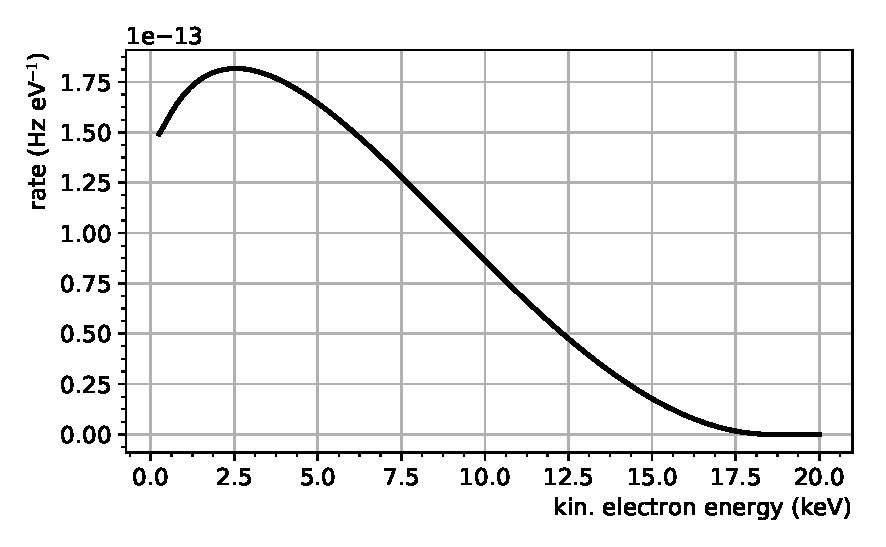
\includegraphics[width=\textwidth]{\currentFigureFolder/diffSpec.pdf}
	\xcaption{Tritium-$\upbeta$ spectrum for a vanishing and non-vanishing neutrino mass}{Tritium-$\upbeta$ spectrum for a vanishing and non-vanishing neutrino mass.}{The plot shows the differential rate as described by equation \eqref{eq:intSpecModelDiffSpec} for a vanishing and non-vanishing neutrino mass. (The spectrum was calculated using the SSC software framework, see section \ref{sec:statMethodsKaFitSSC}, neglecting the sum over the final molecular states.) The inset zooms into the endpoint region where a non-vanishing mass causes a shift and a distortion of the spectrum.}
	\label{fig:intSpecModelDiffSpec}
\end{figure}


This section presents a quantitative expression for the $\upbeta$-decay rate of a tritium molecule in dependence on the kinetic energy of the emitted $\upbeta$ electron (differential rate). Accordingly, the differential rate is depicted in figure~\ref{fig:intSpecModelDiffSpec} for a vanishing and non-vanishing effective electron-antineutrino mass. The following paragraphs describe the differential rate in a top-down approach. In other words, first the whole expression is denoted, then its components are explained.

Using Fermi theory and Fermi's golden rule the decay rate of a tritium molecule is~\cite{Kleesiek2019} 
\begin{align}
\label{eq:intSpecModelDiffSpec}
\diffRate = &
\frac{\fermiConst^2 \abs{V_\mathrm{ud}}^2}{2 \pi^3}
\abs{\nucMatrixElement}^2 \cdot
F(Z, \Esource) \cdot 
p(\Esource+m_\elecIndex) \cdot 
\sum_{f} 
	P_f \cdot 
	\epsilon_f \cdot 
	\sqrt{\epsilon_f^2-\nuMass^2} \cdot 
	\thetaFunc(\epsilon_f-\nuMass)
	\fullstop
\end{align}
Its constituents are the kinetic electron energy $\Esource$;
the effective electron-antineutrino mass $\nuMass$ defined via the PMNS matrix $U$, equation \eqref{eq:PMNSmatrix},
\begin{equation}
	 \nuMass^2 = \abs{U_{\elecIndex i}}^2 m_i^2\,;
\end{equation}
the Fermi constant $\fermiConst$;
the up-down-quark-coupling given by the Cabibo angle $\theta_\mathrm{C}$~\cite{Kleesiek2019}
\begin{equation}
V_\mathrm{ud} = \cos \theta_\mathrm{C} = 
0.97425\pm0.00022;
\end{equation}
and the nuclear transition matrix element~\cite{Kleesiek2019}
\begin{equation}
\abs{\nucMatrixElement}^2 = g_V^2+3g_A^2 \quad
\text{with } g_v = 1 \quad
\text{and} \quad g_A/g_V = -1.2646 \pm 0.0035
\end{equation}
which is independent of the electron's kinetic energy as the decay is super-allowed and given by the vector $g_V$ and axial vector $g_A$ coupling.

Furthermore, the Fermi function $F(Z,\Esource)$ accounts for the Coulomb interaction between the outgoing electron and the daughter nucleus with atomic charge $Z=2$, which in its relativistic version can be approximated as~\cite{Kleesiek2019}
\begin{equation}
F(Z,\Esource) \approx \frac{2 \pi \eta}{1-\exp{2 \pi \eta}} \cdot R
\comma
\end{equation}
with Sommerfeld parameter $\eta = \alpha Z / \beta$, fine structure constant $\alpha$, relativistic velocity $\beta$ and a relativistic correction factor $R = 1.002037-0.001427\beta$~\cite{Kleesiek2019}.

The phase-space factor of the outgoing electron with momentum $p$ and mass $m_\elecIndex$ is given by the factor $p(\Esource+m_\elecIndex)$.

The phase space factor of the emitted neutrino  depends on multiple quantities: First, there is the $\upbeta$-spectrum endpoint $E_0$. $E_0$ is the total nuclear tritium-decay energy $Q$ corrected for the nucleus recoil $E_\mathrm{rec}$ also called endpoint of the $\upbeta$ spectrum
\begin{equation}
\label{eq:intSpecModelEndpoint}
E_0 = Q-E_\mathrm{rec}
\fullstop
\end{equation}
$Q$ is the mass difference of mother and daughter nucleus and was determined in a Penning trap measurement to be $Q=\SI{18592.01\pm0.007}{eV}$~\cite{Myers2015}. Furthermore, there is the final state energy of the molecular system $V_f$. The exited energy state $f$ is caused by vibration, rotation or electronic excitation of the decaying molecule. A review on tritium molecular final states and tabulated values can e.\,g.~be found in~\cite{Bodine2015} and references therein.  The probability that the molecular system is in a final state of energy $V_f$ after the decay is denoted by $P_f$. Then the energy of the neutrino reads 
\begin{equation}
\epsilon_f = E_0 - E - V_f 
\fullstop
\end{equation}
The neutrino's momentum is $\sqrt{\epsilon_f^2-\nuMass^2}$. And the complete phase space factor of the neutrino is a sum over all possible molecular final states labeled $f$.

Lastly, the Heavyside step function $\thetaFunc$ ensures a positive kinetic energy of the neutrino.

\section{Response Function}
The aim of this chapter is the derivation of a formula for the electron rate at the KATRIN detector. Section~\ref{sec:intSpecModelDiffSpec} derived the $\upbeta$-electron rate in dependence of the $\upbeta$-electron energy. The next step is the inclusion of the characteristics of the KATRIN experimental setup. This can be accomplished by denoting the so-called KATRIN response function. It reflects the probability of an $\upbeta$ electron emitted in the \gls{wgts} to reach the KATRIN detector~\cite{Groh2015}.

Within this section the formalism for the KATRIN response function is developed in a bottom-up approach. First, central concepts and the nomenclature are presented in section~\ref{sec:intSpecModelResponseConcepts}. Then, components of the response function are introduced: 
\begin{itemize}
	\item The gas dynamics within the \gls{sts} need to be simulated. See section~\ref{sec:intSpecModelResponseGasDynamics}.
	\item The characteristics of the KATRIN spectrometer can be summarized in the so-called transmission function. See section~\ref{sec:intSpecModelResponseTransmission}.
	\item The passage of electrons through the \gls{wgts} is characterized by scattering from gas molecules. The probability for such scattering is discussed in section~\ref{sec:intSpecModelResponseScattering}. Furthermore, the amount of energy an electron loses when scattering is considered in section~\ref{sec:intSpecModelResponseEloss}.
\end{itemize}
Finally, the described components will be assembled to the KATRIN response function in section~\ref{sec:intSpecModelResponseReconciliation}.
\subsection{Concepts and Nomenclature}
\label{sec:intSpecModelResponseConcepts}
\todo{introduction}

\paragraph{Coordinate System}
This chapter focuses on a one-dimensional description of the KATRIN response function. The position along the beam line is denoted with $z$. The origin of the coordinates system is the center of the \gls{wgts} as already chosen in previous works, e.\,g.~\cite{Groh2015,Kleesiek2014}. In this sense, the start and the end of the \gls{wgts} of length $d$ have the coordinates $\mp d/2$.

\paragraph{Pitch Angle}
Within this chapter the angle between a $\upbeta$ electron's direction of motion and the beam line axis, the so-called pitch angle, is denoted by $\theta$.

\paragraph{Parameter Indices}
Whether a $\upbeta$ electron reaches the KATRIN detector i.\,a.~depends on its parameters when originating in the \gls{wgts}. Within this chapter these starting parameters are denoted with a lower index $\mathrm{S}$. The three decisive starting parameters are the following:
\begin{enumerate}
	\item The starting kinetic energy $\Esource$. It is discussed within the description of the differential rate in equation~\eqref{eq:intSpecModelDiffSpec}.	
	\item The starting position $\zSource$ within the \gls{wgts}.
	\item The starting pitch angle $\thetaSource$ within the \gls{wgts}.
\end{enumerate}
Parameters that denote quantities in the analyzing plane (see section~\ref{sec:katrinExpSetupSpectrometer}) are denoted with a lower index $\mathrm{A}$.

\paragraph{Probabilistic Treatment of  the Starting Pitch Angle}
It should be noted, that the three listed starting parameters are not known for a single $\upbeta$ electron, which suggests a probabilistic treatment. Within the scope of this thesis this is of importance with respect to the starting starting pitch angle. Therefore, the concept is explained in the following:

The mean value of any function $g(\thetaSource)$ depending on a fixed starting pitch angle $\thetaSource$ can be extracted within an interval $[0, \thetaMax]$ given the distribution $\omega(\thetaSource)$ by applying the definition of the mean value
\begin{equation}
\label{eq:intSpecModelPitchAngleAveraging}
\mean{g(\thetaSource)} = 
\frac{
	\int_{0}^{\thetaMax} 
	\omega(\thetaSource)
	g(\thetaSource)
	\d \thetaSource   
}{
	\int_{0}^{\thetaMax} 
	\omega(\thetaSource)
	\d \thetaSource 
} \fullstop
\end{equation}

An isotropic $\upbeta$ electron emission by a tritium molecule into the unit sphere, meaning all combinations of spherical emission angles $(\varphi, \vartheta=\thetaSource)$ are equally likely, yields as distribution for their starting pitch angle\cite{Angrik:2005ep}
\begin{equation}
\omega(\thetaSource) = \sin\thetaSource
\end{equation}
with normalization
\begin{equation}
	\int_{0}^{\thetaMax} 
	\omega(\thetaSource)
	\d \thetaSource = 
	\frac{1}{1-\cos\thetaMax}
	\fullstop
\end{equation}
Within this chapter $\thetaMax$ denotes the maximum acceptance angle due to the magnetic bottle effect as explained in section~\ref{sec:katrinExpSetupSpectrometerMACE} with a design value of $\thetaMax\approx\SI{51}{\degree}$ \cite{Angrik:2005ep}.

\paragraph{Experimental Settings}
As the response function models the characteristics of the KATRIN apparatus it naturally depends on the experimental settings. The quantities used within this chapter are listed in the following:
\begin{itemize}
	\item the magnetic field $\Bsource$ at the place of origin of a $\upbeta$ electron within the \gls{wgts};
	\item the magnetic field $\Bana$ within the analyzing plane;
	\item the maximum magnetic field $\Bmax$ along the beam line axis;
	\item the retarding voltage $U$ and the retarding energy $qU$;
	\item the starting potential $\Usource$ of a $\upbeta$ electron within the \gls{wgts}.
\end{itemize}
For the detailed meaning of these parameters and their KATRIN design values, see section \ref{sec:katrinExpSetupSpectrometer}.
It should be noted, that none of these quantities are constant, but they exhibit a spatial, especially a radial, dependency~\cite{Angrik:2005ep}. For ease of notation, the spatial dependency is left implicit within this chapter.


\subsection{Gas Dynamcis}
\label{sec:intSpecModelResponseGasDynamics}
The gas dynamics within the \gls{sts} have to be simulated. This topic is not treated in detail within this thesis. Instead the reader is referred to~\cite{Hoetzel2012}. In short, in a one-dimensional description the output of such a gas dynamic simulation is the gas molecule density $\rho(z)$. Averaged over all starting positions $z$ and multiplied with the length $d$ of the \gls{wgts}, one obtains the design column density $\rho d = \SI{5e17}{cm^{-2}}$~\cite{Angrik:2005ep}.

\subsection{Transmission Function}
\label{sec:intSpecModelResponseTransmission}
\begin{figure}
	\centering
	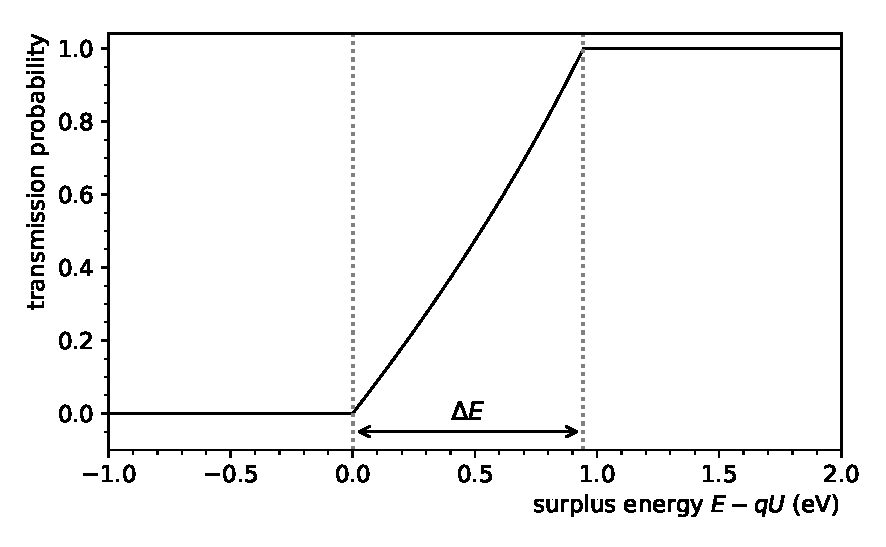
\includegraphics[width=\textwidth]{\currentFigureFolder/transmission.pdf}
	\xcaption{The KATRIN transmission function}{The KATRIN transmission function}{as described by equation \eqref{eq:intSpecModelTransmission}. It denotes the probability for an $\upbeta$ electron with a kinetic energy $E$ to pass through the spectrometer set to a retarding potential of $U$. The probabilistic treatment of the starting pitch angles of $\upbeta$ electrons leads to the \gls{mace}-filter width $\Delta E$. (The transmission function was calculated using the SSC software framework, see section \ref{sec:statMethodsKaFitSSC}.) }
	\label{fig:intSpecModelTransmission}
\end{figure}
The transmission function denotes the probability of a $\upbeta$ electron to pass the \gls{mace} filter. It can be characterized by the so-called transmission energy~\cite{Groh2015}
\begin{equation}
\label{eq:intSpecModelTransmissionEnergy}
\Etrans = 
\frac{
	q(U-\Usource)
}{
	1-\sin^2\thetaSource \frac{\Bana}{\Bsource} \frac{\gammaSource+1}{\gammaAna+1}
}
\fullstop
\end{equation}
where $\gammaSource\equiv\gammaSource(\Esource)$ and $\gammaAna$ denote the relativistic $\gamma$-factor of the $\upbeta$ electrons at their place of origin respectively the analyzing plane. As the electrons are slowed down substantially by the retarding potential in the spectrometer, it holds $\gammaAna\approx1$~\cite{Groh2015}. In the following, for ease of notation, also $\Usource=0$ and $\gammaSource=1$ is assumed.

$\upbeta$ electrons pass the \gls{mace} filter if their energy $E$ when arriving at the spectrometer surpasses the transmission energy $\EtransPure$. This condition can be resolved for the starting pitch angle~\cite{Groh2015}
\begin{align}
&E > \Etrans \nonumber \\
\Leftrightarrow \quad
& \thetaSource < \thetaTrans
\coloneqq
\arcsin
\left(\sqrt{
	\frac{E-qU}{E} 
	\frac{\Bana}{\Bsource}
}\right)
\fullstop
\label{eq:intSpecModelTransmissionPitchAngle}
\end{align}
Using equation \eqref{eq:intSpecModelTransmissionPitchAngle}, the transmission function depending on the starting pitch angle and the starting energy of $\upbeta$ electrons can be formulated as a step function
\begin{equation}
\label{eq:intSpecModelTransmissionStep}
\mathcal{T}(E, qU, \thetaSource) =
\begin{cases}
1 & \text{if } \thetaSource < \thetaTrans \\
0 & \text{otherwise} 
\end{cases}
\fullstop
\end{equation}
Calculating the mean value of this step function with respect to the probabilistic distributed starting pitch angles of $\upbeta$ electrons as described in section~ \ref{sec:intSpecModelResponseConcepts} yields the often quoted KATRIN transmission function~\cite{Angrik:2005ep}
\begin{equation}
\label{eq:intSpecModelTransmission}
	T(E, qU) = 
	\mean{\mathcal{T}(E, qU, \thetaSource)} =
	\begin{cases}
	0 & \text{ if } E < qU \\
	\frac{
		1-\sqrt{
			1-\frac{E-qU}{E} 
			\frac{\Bsource}{\Bana}
		} 
	}{
		1-\sqrt{1-\frac{\Delta E}{E}\frac{\Bsource}{\Bana}}
	}
	& \text{ if } qU < E < qU + \Delta E \\
	1 & \text{ if } qU + \Delta E < E
	\end{cases}
	\comma
\end{equation}
where $\Delta E=E\cdot\Bana/\Bmax$ is the \gls{mace}-filter width as explained in section~\ref{sec:katrinExpSetupSpectrometer}. The transmission function is depicted in figure~\ref{fig:intSpecModelTransmission} for the KATRIN design values.

\subsection{Probability of Electron Scattering within the \gls{wgts}}
\label{sec:intSpecModelResponseScattering}
This section aims at deriving an expression for the probability $P_l$ of an electron to scatter $l$ times within the \gls{wgts} in a bottom-up approach.

First, an expression for the effective column density $\lambda$ an electron passes through is presented. The electron moves on a spiral track due to its cyclotron motion in the magnetic field in the \gls{wgts}. Therefore, when traveling an infinitesimal distance $\d z$ in $z$-direction, it travels a total distance of
\begin{equation}
\label{eq:intSpecModelInfinitesimalElecPath}
\d s = \frac{1}{\cos\thetaSource} \d z 
\fullstop
\end{equation}
(It is noteworthy, that is expression is independent of the electron energy and the magnetic field strength in the \gls{wgts}.)
The effective column density can then be expressed as a path integral over the gas density~$\rho(z)$ from the starting position of the electron to the point where it leaves the \gls{wgts}
\begin{equation}
\label{eq:intSpecModelEffColumnDensity}
\lambda(\zSource,\thetaSource) = 
\int_{\varphi} \rho(\Vec{r})\d s =
\frac{1}{\cos\thetaSource}
\int_{\zSource}^{d/2} \rho(z)\d z
\fullstop
\end{equation}
The expected scattering count then is the product of the effective column density $\lambda(\zSource,\thetaSource)$ and the scattering cross section $\sigma$~\cite{Groh2015}
\begin{equation}
\label{eq:intSpecModelExpectedScatteringCount}
\mu(\zSource, \thetaSource) = \lambda(\zSource,\thetaSource) \sigma \fullstop
\end{equation}
The scattering process fulfills the conditions of a Poisson process, namely scattering once does quasi not influence the probability of an electron to scatter again; the expected scattering count $\mu(\zSource, \thetaSource)$ stays constant (under the assumptions made so far); and it is unlikely for two scatterings to happen within a short distance. Thus, the probability for $l$-fold scattering can be expressed as a Poisson distribution~\cite{Groh2015}
\begin{equation}
\label{eq:scatProbs}
P_l(\zSource, \thetaSource) = 
\frac{
	\mu(\zSource, \thetaSource)^l
}{l!}
\mathrm{e}^{-\mu(\zSource, \thetaSource)} \fullstop
\end{equation}
The mean value with respect to the starting positions and the starting pitch angles can be calculated~\cite{Groh2015}
\begin{equation}
	\label{eq:intSpecModelAveragedScatProbs}
	\bar{P}_l =
	\frac{1}{d}
	\int_{-d/2}^{d/2}
		\frac{1}{1-\cos\thetaMax}
		\int_{0}^{\thetaMax}
			\sin\thetaSource
			P_l(\zSource,\thetaSource)
		\d \thetaSource
	\d \zSource
	\fullstop
\end{equation}
Table~\ref{tab:intSpecModelAveragedScatProbs} lists the numerical evaluation of these averaged scattering probabilities.

\begin{table}[ht]
	\centering
	\xcaption{Averaged probability for electron scattering within the \gls{wgts}}{Averaged probability for electron scattering within the \gls{wgts}.}{Listed are the evaluations of equation \eqref{eq:intSpecModelAveragedScatProbs} for the following input parameters:
	A scattering cross section of $\sigma=\SI{3.456e-22}{m^2}$~\cite{Angrik:2005ep},
	a constant gas column density $\rho d = \SI{5e17}{cm^{-2}}$, 
	a \gls{wgts} length of $d=\SI{10.0820}{m}$
	and a maximum acceptance angle of $\thetaMax=\SI{50.7685}{\degree}$.
	The same values can be found in \cite{Groh2015, Kleesiek2014}.}
	\begin{tabular}{cr}
		\toprule
		\makecell[tl]{scattering count $l$} &
		\makecell[tl]{scattering probability\\ according to equation \eqref{eq:intSpecModelAveragedScatProbs}}\\
		\hline
		0 & 41.33\,\SI{}{\percent }\\
		1 & 29.27\,\SI{}{\percent} \\
		2 & 16.73\,\SI{}{\percent} \\
		3 &  7.91\,\SI{}{\percent} \\
		4 &  3.18\,\SI{}{\percent} \\
		\bottomrule
	\end{tabular}
	\label{tab:intSpecModelAveragedScatProbs}
\end{table}

\subsection{Energy Loss of Electrons due to Scattering}
\label{sec:intSpecModelResponseEloss}
This section describes the so called ``energy loss function'' $f_l(\epsilon)$. It denotes the probability of an electron to loose an energy $\epsilon$ when scattering $l$ times. Only the case of inelastic scattering is treated here. For an additional treatment of elastic scattering, that is less likely by one order og magnitude, the reader is referred to~\cite{Kleesiek2019}.

A phenomenological description for 1-fold scattering of electrons from hydrogen isotopologues was derived at the Troitsk experiment~\cite{Aseev2000, Abdurashitov2017}
\newcommand{\epsCrit}{\epsilon_\mathrm{c}}
\begin{equation}
	f_1(\epsilon) =
	\begin{cases}
		A_1 
		\euler^{ 
			-2\left(
			\frac{\epsilon-\epsilon_1}{\omega_1}
			\right)^2
		}
		&\text{ if } \epsilon < \epsCrit \\
		A_2\frac{
			\omega_2^2
		}{
			\omega_2^2+4(\epsilon-\epsilon_2)^2
		} 
		&\text{ if } \epsilon \geq \epsCrit
	\end{cases}
\end{equation}
with the parameters 
$A_1=0.204\pm0.0001$, 
$A_2=0.204\pm0.0001$, 
$\omega_1=\SI{1.85\pm0.02}{eV}$
$\omega_2=\SI{12.5\pm0.2}{eV}$
$\epsilon_1=\SI{12.6}{eV}$ (fixed)
$\epsilon_2=\SI{14.30\pm0.02}{eV}$




\subsection{Assembling of the Full Response Function}
\label{sec:intSpecModelResponseReconciliation}

\def\currentRootFolder{chapter/modelOfIntegratedRate/neutrinoMassMeasurement}
\def\currentFigureFolder{\currentRootFolder/fig}
\newcommand{\elecIndex}{\mathrm{e}}

\newcommand{\Bsource}{B^j_\mathrm{S}}
\newcommand{\BsourceAvg}{B_\mathrm{S}}
\newcommand{\zSource}{z_\mathrm{S}}
\newcommand{\thetaSource}{\theta_\mathrm{S}}
\newcommand{\thetaSourceAvg}{\theta_\mathrm{S}}
\newcommand{\Esource}{E_\mathrm{S}}
\newcommand{\Usource}{U^j_\mathrm{S}}
\newcommand{\gammaSource}{\gamma_\mathrm{S}}


\newcommand{\Bps}{B_\mathrm{PS2}}
\newcommand{\Bana}{B_\mathrm{A}}
\newcommand{\Bpinch}{B_\mathrm{P}}
\newcommand{\Bmax}{B_\mathrm{max}}
\newcommand{\Bmin}{B_\mathrm{min}}

\newcommand{\thetaMax}{\theta_\mathrm{max}}
\newcommand{\Esur}{E_\mathrm{sur}}
\newcommand{\detEff}{\epsilon_\mathrm{det}}
\newcommand{\macefilterwidth}{\Delta \mathcal{E}^j(\thetaS^j)}

\newcommand{\EtransPure}{E^j_\mathrm{tr}}
\newcommand{\Etrans}{\EtransPure(qU,\Esource,\thetaSource)}
\newcommand{\thetaTransPure}{\theta^j_\mathrm{tr}}
\newcommand{\thetaTrans}{\thetaTransPure(\Esource,qU)}

\newcommand{\As}{A_\mathrm{S}}
\newcommand{\Rbg}{R_\mathrm{bg}}


\newacronym{standardmodel}{SM}{Standard Model of Particle Physics}
\newacronym{lep}{LEP}{Large Electron Positron Collider}
\newacronym{ssm}{SSM}{standard solar model}

\section{A KATRIN Neutrino Mass Measurement}
\label{sec:katrinExpNuMassMeasurement}
\todo{Introduction}
The predicted counts for a retarding energy of $qU$ when measuring a duration $t(qU)$ are
\begin{equation}
\label{eq:intSpecModelCountsFinal}
\bar{N}(qU) = t(qU) \cdot \detEff \cdot \left(
\As \cdot
\sum_{j}
N_T^j \cdot
\int_{qU}^{E_0} 
\left(\frac{\d \Gamma(\Esource)}{ \d \Esource}\right) \cdot 
\bar{R}^j(\Esource, qU) 
\d \Esource +
\Rbg
\right)
\fullstop
\end{equation}
Here, $\As=1$ is a normalization factor, $\detEff \in [0,1]$ is the detector efficiency \todo{reference KATRIN chapter}, the sum goes over all source slices with label $j$, $N_T^j$ is the number of tritium molecules in the $j$th source slice, $\left(\d \Gamma(\Esource) / \d \Esource \right)$ is the differential rate from \eqref{eq:intSpecModelDiffSpec}, $\bar{R}^j(\Esource, qU)$ is the response function from \eqref{eq:} and $\Rbg$ is the rate of background events.

KATRIN measures electron counts as described in \eqref{eq:countsSCCFinal} at a set of retarding energies ${qU_i}$. How much measurement time $t(qU_i)$ is attributed to a certain retarding energy is called a \gls{mtd}. The \gls{mtd} influences the experiment's sensitivity to the neutrino mass. An optimal \gls{mtd} balances the following aspects:
\begin{enumerate}
	\item Some measurement time has to be attributed to retarding energies beyond the endpoint of the spectrum to determine the background rate. The optimal duration depends on the background rate.
	\item The shape of the integral tritium $\upbeta$ spectrum depends the strongest on the neutrino mass near its endpoint $E_0$ \eqref{eq:endpoint}. \todo{Plot!}
	\item Measurements deeper into the spectrum increase the count rate and hence, lower the statistical uncertainty due to Poisson statistics.
	\item The theoretical description of the integral tritium $\upbeta$ spectrum is optimized for the endpoint region. Deeper scans introduce modeling uncertainties.
\end{enumerate}
The KATRIN Design Report \cite{Angrik:2005ep} suggests 5 \gls{mtd}s for different measurement ranges $[E_0-\alpha\;\SI{}{eV}, E_0 + \SI{5}{eV}]$ with $\alpha \in \{20, 25, 30, 40, 50\}$ and the conclusion that $\alpha=30$ yields the best sensitivity to the neutrino mass. Furthermore, searches for sterile neutrinos at the keV-scale would require deeper scans~\cite{Kleesiek2014}. Several measurement campaigns were already conducted. The \gls{ft} commissioning campaign successfully proved the apparatus functioning. The corresponding \gls{mtd} covered a range starting at $\sim E_0-\SI{1.6}{keV}$. The \gls{knm1} campaign is evaluated during the writing of this thesis. It set out to establish an unprecedented limit on the neutrino mass by $\upbeta$-decay measurements. Its \gls{mtd} starts at $\sim E_0-\SI{90}{eV}$.